\documentclass[12pt, stu, abstract]{apa7}

% ------------------------------------------------
% Standard packages
% ------------------------------------------------
\usepackage[american]{babel}
\usepackage{csquotes}
\usepackage[style=apa,sortcites=true,sorting=nyt,backend=biber]{biblatex}
\DeclareLanguageMapping{american}{american-apa}
\addbibresource{references.bib} 

\usepackage{amsmath}
\usepackage{amssymb}
\usepackage{mathtools}
\usepackage{bm}

\usepackage{booktabs}
\usepackage{graphicx}
\usepackage{float}
\usepackage{caption}
\usepackage{subcaption}

\usepackage{enumitem}
\setlist[itemize]{itemsep=0pt,topsep=0pt,parsep=0pt}

\usepackage{siunitx}
\usepackage{threeparttable}

\usepackage{appendix}

\usepackage{hyperref}
\hypersetup{
    colorlinks=true,
    linkcolor=blue,
    filecolor=magenta,
    urlcolor=cyan,
}


% ------------------------------------------------
% Metadata
% ------------------------------------------------
\title{The Impact of Interest-Rate Changes on Sector Stocks and Sun-Belt Real-Estate Markets}
\author{Daniel Lott}
\authorsaffiliations{University of Arizona}
\course{MATH 462 Financial Mathematics}
\professor{Dr. Lianfen Qian}
\duedate{May 14, 2025}
\abstract{This study investigates the relationship between Federal Reserve interest rate changes and financial markets, focusing on sector equity performance and real estate dynamics in Sun Belt states. Using time series data from 2006-2025, including sector ETFs, Federal Funds Rate, mortgage rates, and Zillow Home Value Index data, the analysis employs regression models to quantify market sensitivities to rate changes. Key findings reveal heterogeneous sector responses, with Energy showing positive sensitivity to rate increases while Technology exhibits negative correlation. Housing markets demonstrate varying lag structures, with Arizona responding immediately to rate changes while Florida shows delayed effects. Financial mathematics applications include cash flow modeling demonstrating how each 1\% mortgage rate increase reduces IRR by approximately 0.146-0.147 percentage points. These results offer actionable insights for sector rotation strategies and regional real estate investment decisions during monetary policy shifts.}
\keywords{interest rates, sector rotation, NPV, IRR, housing markets, Federal Reserve}

% ------------------------------------------------
% Document
% ------------------------------------------------
\begin{document}
\maketitle

Fed policy plays a crucial role in pricing risk assets across financial markets. Changes in interest rates influence both equity valuations and real estate markets through multiple transmission mechanisms. Early research by \textcite{bernanke2005} established that unexpected Federal Funds Rate changes significantly impact stock market returns, with this relationship varying substantially across economic sectors. Subsequent work by \textcite{giuliodori2005} demonstrated that housing markets exhibit heterogeneous responses to monetary policy based on region-specific factors.

This study addresses three primary research questions: (1) How do changes in Federal Reserve interest rates impact stock market returns across different sectors? (2) What is the relationship between interest rate changes and real estate markets, particularly in states with high population growth like Florida and Arizona? (3) How can financial mathematics concepts such as rate of return, NPV, and IRR be applied to analyze these relationships?

The research contributes to existing literature by integrating traditional econometric analysis with applied financial mathematics to quantify investment implications. By examining sector-specific equity responses alongside regional housing market dynamics, this study provides both theoretical insights and practical guidance for investors navigating changing interest rate environments. \footnote{All code and data processing scripts used in this analysis are available at: \url{https://github.com/Dmeisterr/462-Final-Project}}

\section{Data}
\subsection{Data Sources}
The analysis relied on four primary types of financial time series data spanning from 2006 to 2025:

\begin{itemize}
\item \textbf{Sector ETFs:} Daily price data for 10 SPDR sector ETFs (XLB, XLU, XLV, XLE, XLF, XLP, XLRE, XLK, XLI, XLY) representing distinct segments of the US equity market. These ETFs track the performance of S\&P 500 companies grouped by industry sector.

\item \textbf{Federal Funds Rate (FFR):} Monthly effective Federal Funds Rate data from the Federal Reserve Economic Data (FRED) database, reflecting the central bank's monetary policy stance.

\item \textbf{Mortgage Rates:} Weekly 30-year fixed mortgage rate data (MORTGAGE30US series) from FRED, representing the borrowing costs for residential real estate.

\item \textbf{Zillow Home Value Index (ZHVI):} Monthly housing price data for Arizona and Florida, chosen as representative Sun Belt states with high population growth during the study period.
\end{itemize}

\subsection{Data Processing}
Data cleaning and integration were performed using a structured workflow in DataCleaning.ipynb:

\begin{itemize}
\item \textbf{Collection \& Standardization:} Raw CSV files were standardized to a consistent date format with Python's pandas library.

\item \textbf{Frequency Harmonization:} Higher-frequency data (daily stock prices) were downsampled to monthly observations using end-of-month values to align with the lower-frequency macroeconomic indicators.

\item \textbf{Forward-Fill Imputation:} For any date gaps in lower-frequency data (e.g., weekly mortgage rates), values were forward-filled to ensure consistent daily observations across the merged dataset.

\item \textbf{Data Transformation:}
\begin{itemize}
    \item First differences of FFR and mortgage rates ($\Delta$FFR, $\Delta$Mortgage30Y) to capture rate changes
    \item Percentage returns for sector ETFs and ZHVI values to enable comparable analysis
\end{itemize}
\end{itemize}

\subsection{Final Dataset Structure}
The resulting combined\_data\_final.csv contains the following columns:

\begin{itemize}
\item Date: Daily timestamps serving as the index
\item Sector ETF columns (XLB, XLU, etc.): Daily closing prices for each sector
\item FFR: Federal Funds Rate (percentage)
\item Mortgage30Y: 30-year fixed mortgage rate (percentage)
\item Florida\_ZHVI and Arizona\_ZHVI: Housing price indices
\end{itemize}

For analysis in DataAnalysis.ipynb, this dataset was further manipulated to:
\begin{itemize}
\item Calculate return series for all asset classes
\item Align time series for regression analysis
\item Create lagged variables to study lead-lag relationships between interest rates and asset returns
\end{itemize}

The final dataset contains 4,623 daily observations spanning 19 years, providing comprehensive coverage of multiple interest rate cycles.

\section{Methodology}
\subsection{Equity Sector Analysis}
To quantify the relationship between Federal Reserve policy changes and equity sector performance, I implemented a multi-faceted regression approach:

\textbf{Baseline OLS Models:} First-difference regressions were constructed between month-over-month Federal Funds Rate changes ($\Delta$FFR) and monthly sector ETF returns. These models captured the contemporaneous sensitivity of sectors to interest rate adjustments using the equation:

\begin{equation}
R_{sector,t} = \alpha + \beta \Delta \text{FFR}_t + \varepsilon_t
\end{equation}

where $\beta$ represents the sector's rate sensitivity coefficient. Statistical significance was evaluated using t-tests with heteroskedasticity-robust standard errors.

\textbf{Confidence Interval Estimation:} 95\% confidence intervals were computed for all beta coefficients using the t-distribution with n-2 degrees of freedom to assess statistical significance and precision of estimates. For each sector ETF, the formula applied was:

\begin{equation}
\text{CI}_{95\%} = \beta \pm t_{0.975,n-2} \times \text{SE}_{\beta}
\end{equation}

\textbf{Lead-Lag Analysis:} To investigate delayed market reactions, I constructed lagged regressions across four time horizons (0, 1, 2, and 3 months). This approach allowed identification of sectors where rate effects materialize gradually rather than immediately, using models of the form:

\begin{equation}
R_{sector,t} = \alpha + \beta \Delta \text{FFR}_{t-k} + \varepsilon_t
\end{equation}

where $k$ represents the lag period in months.

\subsection{Housing Market Analysis}
The housing analysis employed distributed-lag models to capture the dynamic relationship between interest rate changes and home price movements in Florida and Arizona:

\textbf{Dual Rate Variables:} Both Federal Funds Rate changes ($\Delta$FFR) and 30-year mortgage rate changes ($\Delta$Mortgage) were analyzed as explanatory variables to distinguish between policy rate and consumer financing rate effects.

\textbf{Extended Lag Structure:} Given the slower adjustment mechanisms in real estate markets, I implemented a longer lag structure (0, 3, 6, 9, and 12 months) compared to equity markets. This captured temporal dynamics using the model:

\begin{equation}
R_{ZHVI,t} = \alpha + \sum_{k=0}^{12} \beta_k \Delta \text{Rate}_{t-k} + \varepsilon_t
\end{equation}

where $\Delta \text{Rate}$ represents either $\Delta$FFR or $\Delta$Mortgage, and $\beta_k$ is the sensitivity coefficient at lag $k$.

\textbf{State Comparison Framework:} Parallel analyses for Florida and Arizona enabled direct comparison of rate sensitivities between these demographically similar but potentially financially distinct housing markets.

\subsection{NPV and IRR Cash Flow Modeling}
To translate interest rate impacts into actionable investment metrics, I developed a parametric cash flow model for residential real estate investments:

\textbf{Model Specification:} The model incorporated key parameters including:
\begin{itemize}
\item Loan-to-value ratio: 80\%
\item Gross rental yield: 6\% annually
\item Operating expenses: 25\% of gross rental income
\item Investment horizon: 5 years
\item Discount rate for NPV: 5\% annually
\end{itemize}

\textbf{Scenario Analysis:} Three mortgage rate scenarios (3\%, 5\%, and 7\%) were evaluated to quantify the impact of varying interest costs on investment returns. The cash flow vector for each scenario was constructed as:

\begin{align}
\text{CF}_0 &= -\text{ Down payment (initial investment)} \\
\text{CF}_1 \ldots \text{CF}_{59} &= \text{ Monthly net rental income - mortgage interest} \\
\text{CF}_{60} &= \text{ Final month's net rental income - mortgage interest + property sale proceeds}
\end{align}

\textbf{Return Metrics:} For each scenario, both Net Present Value (NPV) and Internal Rate of Return (IRR) were calculated:

\begin{equation}
\text{NPV} = \sum_{t=0}^{60} \frac{\text{CF}_t}{(1+r)^{t/12}}
\end{equation}

where $r$ represents the annual discount rate (5\%), and

\begin{equation}
\text{IRR} = r \text{ such that } \sum_{t=0}^{60} \frac{\text{CF}_t}{(1+r)^{t/12}} = 0
\end{equation}

This comprehensive methodology enabled quantification of interest rate sensitivities across both equity and real estate markets, while the cash flow modeling translated these sensitivities into practical investment metrics.

\section{Results}
\subsection{Sector ETF Sensitivity to Federal Funds Rate Changes}

The regression analysis revealed substantial heterogeneity in how different equity sectors respond to Federal Funds Rate (FFR) changes, as illustrated in Figure~\ref{fig:sector_sens} and summarized in Table~\ref{tab:sector_betas}. Energy (XLE) demonstrated the strongest positive sensitivity with a beta coefficient of 0.063, while Technology (XLK) exhibited a negative relationship with a beta of -0.031. However, none of the sectors showed statistically significant responses at the 95\% confidence level, as all confidence intervals crossed zero (Table~\ref{tab:sector_ci}).

\begin{table}[htbp]
\centering
\caption{Sector ETF Sensitivities to Federal Funds Rate Changes}
\label{tab:sector_betas}
\begin{tabular}{lrr}
\toprule
Sector & $\beta$ (slope) & $R^2$ \\
\midrule
XLE & 0.062909 & 0.015808 \\
XLI & 0.028707 & 0.008898 \\
XLF & 0.027465 & 0.007257 \\
XLU & 0.008942 & 0.001541 \\
XLRE & 0.002812 & 0.000105 \\
XLB & -0.005444 & 0.000307 \\
XLP & -0.005595 & 0.000902 \\
XLV & -0.022827 & 0.010038 \\
XLY & -0.023943 & 0.005509 \\
XLK & -0.031457 & 0.010444 \\
\bottomrule
\end{tabular}
\end{table}

\begin{table}[htbp]
\centering
\caption{95\% Confidence Intervals for Sector Beta Coefficients}
\label{tab:sector_ci}
\begin{tabular}{lrrr}
\toprule
Sector & $\beta$ & Lower 95\% CI & Upper 95\% CI \\
\midrule
XLE & 0.062909 & -0.030026 & 0.155844 \\
XLI & 0.028707 & -0.028016 & 0.085429 \\
XLF & 0.027465 & -0.032677 & 0.087606 \\
XLU & 0.008942 & -0.033677 & 0.051561 \\
XLRE & 0.002812 & -0.048621 & 0.054244 \\
XLB & -0.005444 & -0.063595 & 0.052707 \\
XLP & -0.005595 & -0.040459 & 0.029269 \\
XLV & -0.022827 & -0.065267 & 0.019613 \\
XLY & -0.023943 & -0.084170 & 0.036284 \\
XLK & -0.031457 & -0.088783 & 0.025869 \\
\bottomrule
\end{tabular}
\end{table}

The explanatory power of FFR changes was notably limited across all sectors, with $R^2$ values below 2\%. The highest $R^2$ value was for XLE at 1.58\%, followed by XLK at 1.04\%. This suggests that while monetary policy shifts may influence sector returns, they represent just one of many factors affecting equity performance.

The lag structure analysis revealed dynamic patterns in how sectors process interest rate information (see Figure~\ref{fig:sector_lagged} and Table~\ref{tab:sector_lags}). Most sectors exhibit their strongest reaction to FFR changes at lag 0 (contemporaneous effect), with these effects generally dissipating or reversing by lag 3. Notably, the Financial sector (XLF) displayed a sign reversal from lag 0 ($\beta = 0.027$) to lag 1 ($\beta = -0.061$), suggesting a rapid reassessment of rate impact. Energy (XLE) showed the most dramatic shift, from $\beta = 0.063$ at lag 0 to $\beta = -0.110$ at lag 1. This pattern supports the hypothesis that equity markets quickly incorporate monetary policy signals, typically within one month.

\begin{table}[htbp]
\centering
\caption{Sector Beta Coefficients with Lagged Federal Funds Rate Changes}
\label{tab:sector_lags}
\begin{tabular}{lrrrrrrrrrr}
\toprule
Lag & XLB & XLU & XLV & XLE & XLF & XLP & XLRE & XLK & XLI & XLY \\
\midrule
0 & -0.005 & 0.009 & -0.023 & 0.063 & 0.027 & -0.006 & 0.003 & -0.031 & 0.029 & -0.024 \\
1 & -0.069 & -0.024 & -0.042 & -0.110 & -0.061 & -0.029 & -0.050 & -0.063 & -0.038 & -0.075 \\
2 & -0.007 & -0.013 & -0.010 & 0.033 & -0.009 & -0.011 & -0.021 & -0.025 & -0.009 & -0.022 \\
3 & 0.013 & -0.009 & 0.000 & 0.061 & 0.021 & -0.003 & -0.003 & -0.006 & 0.021 & -0.005 \\
\bottomrule
\end{tabular}
\end{table}

\subsection{Housing Market Response to Interest Rate Changes}

The analysis of Zillow Home Value Index (ZHVI) returns revealed distinct patterns across states, as shown in Figure~\ref{fig:zhvi_sens} and detailed in Table~\ref{tab:realestate_reg}. Arizona demonstrated immediate negative sensitivity to FFR changes ($\beta = -0.011$), while Florida initially showed positive sensitivity ($\beta = 0.004$) that turned negative at longer lags. These findings suggest that Arizona's housing market reacts more promptly to monetary tightening compared to Florida.

\begin{table}[htbp]
\centering
\caption{Real Estate Sensitivity to Interest Rate Changes}
\label{tab:realestate_reg}
\begin{tabular}{lrrrr}
\toprule
State & $\beta$ ($\Delta$FFR) & $R^2$ ($\Delta$FFR) & $\beta$ ($\Delta$Mortgage) & $R^2$ ($\Delta$Mortgage) \\
\midrule
Florida & 0.004432 & 0.00642 & 0.008643 & 0.047732 \\
Arizona & -0.010853 & 0.02759 & 0.005549 & 0.014096 \\
\bottomrule
\end{tabular}
\end{table}

\begin{table}[htbp]
\centering
\caption{ZHVI Beta Coefficients with Confidence Intervals}
\label{tab:zhvi_ci}
\small
\begin{tabular}{l@{\hspace{0.8em}}r@{\hspace{0.8em}}r@{\hspace{0.8em}}r@{\hspace{0.8em}}r@{\hspace{0.8em}}r@{\hspace{0.8em}}r@{\hspace{0.8em}}r@{\hspace{0.8em}}r}
\toprule
State & $\beta$ $\Delta$FFR & CI\_low & CI\_high & p-val & $\beta$ $\Delta$Mort & CI\_low & CI\_high & p-val \\
\midrule
Florida & 0.004432 & -0.005890 & 0.014754 & 0.3967 & 0.008643 & 0.001415 & 0.015871 & 0.0195 \\
Arizona & -0.010853 & -0.022915 & 0.001210 & 0.0774 & 0.005549 & -0.003139 & 0.014236 & 0.2083 \\
\bottomrule
\end{tabular}
\end{table}

Mortgage rate changes produced stronger statistical relationships than FFR changes, with $R^2$ values of 4.8\% for Florida and 1.4\% for Arizona. Florida's response to mortgage rate changes was statistically significant (p = 0.020) with a confidence interval of [0.001, 0.016], as shown in Table~\ref{tab:zhvi_ci}. This aligns with expectations that consumer mortgage rates have more direct influence on housing markets than policy rates, as evidenced in Figures~\ref{fig:fl_zhvi} and~\ref{fig:az_zhvi}.

Florida's FFR beta coefficient transitions from slightly positive at lag 0 ($\beta = 0.004$) to increasingly negative at lags 6-12 months (reaching $\beta = -0.014$ at lag 12), indicating delayed cooling effects of rate hikes (Figure~\ref{fig:fl_rate_sens} and Table~\ref{tab:ffr_lags}). For mortgage rate sensitivity, both states exhibit increasingly negative betas at longer lags, with Arizona reaching negative sensitivity (-0.009) at lag 12 months (Figure~\ref{fig:az_rate_sens} and Table~\ref{tab:mortgage_lags}).

\begin{table}[htbp]
\centering
\caption{Federal Funds Rate Beta Coefficients at Various Lags}
\label{tab:ffr_lags}
\begin{tabular}{lrr}
\toprule
Lag (months) & Florida & Arizona \\
\midrule
0 & 0.004432 & -0.010853 \\
3 & -0.004215 & -0.020546 \\
6 & -0.007770 & -0.017306 \\
9 & -0.007326 & -0.011393 \\
12 & -0.013750 & -0.017330 \\
\bottomrule
\end{tabular}
\end{table}

\begin{table}[htbp]
\centering
\caption{Mortgage Rate Beta Coefficients at Various Lags}
\label{tab:mortgage_lags}
\begin{tabular}{lrr}
\toprule
Lag (months) & Florida & Arizona \\
\midrule
0 & 0.008643 & 0.005549 \\
3 & 0.005537 & 0.003443 \\
6 & 0.000925 & -0.001327 \\
9 & -0.002591 & -0.007315 \\
12 & -0.004070 & -0.009354 \\
\bottomrule
\end{tabular}
\end{table}

The relationship between Federal Funds Rate and home values across both states is further illustrated in Figure~\ref{fig:zhvi_ffr}, while Figure~\ref{fig:zhvi_mort} shows the corresponding relationship with mortgage rates. These patterns suggest a transmission mechanism where policy rate changes gradually impact housing markets, with full effects taking 6-12 months to materialize.

\subsection{NPV and IRR Analysis of Housing Investment}

The cash flow modeling results quantify how different mortgage rates affect investment returns in both states, as shown in Figure~\ref{fig:irr_mort} and detailed in Table~\ref{tab:npv_irr}. For a 5-year investment horizon starting in January 2020, Arizona properties demonstrated higher NPV values compared to Florida properties across all mortgage rates, while IRR returns were slightly higher for Florida. At a 3\% mortgage rate, the model yielded IRRs of 3.88\% for Florida and 3.85\% for Arizona, while at a 7\% rate, returns declined to 3.30\% and 3.26\% respectively.

\begin{table}[htbp]
\centering
\caption{NPV and IRR Metrics for Various Mortgage Rate Scenarios}
\label{tab:npv_irr}
\begin{tabular}{lrrr}
\toprule
State & Mortgage Rate & NPV & IRR \\
\midrule
Florida & 3\% & \$275,051.08 & 0.038843 \\
Florida & 5\% & \$257,635.23 & 0.035840 \\
Florida & 7\% & \$240,219.38 & 0.032996 \\
Arizona & 3\% & \$303,262.81 & 0.038521 \\
Arizona & 5\% & \$283,631.59 & 0.035499 \\
Arizona & 7\% & \$264,000.36 & 0.032636 \\
\bottomrule
\end{tabular}
\end{table}

\begin{table}[htbp]
\centering
\caption{IRR Sensitivity to Mortgage Rate Changes}
\label{tab:irr_slopes}
\begin{tabular}{lrrrr}
\toprule
State & Slope (\% IRR per 1\% rate) & Intercept & R² & p-value \\
\midrule
Florida & -0.1462 & 4.3201\% & 0.9998 & 0.0099 \\
Arizona & -0.1471 & 4.2909\% & 0.9998 & 0.0099 \\
\bottomrule
\end{tabular}
\end{table}

Regression analysis of IRR sensitivity to mortgage rates revealed slopes of -0.1462\% IRR per 1\% mortgage rate increase for Florida and -0.1471\% for Arizona (both with R² = 0.9998, p = 0.0099), as shown in Table~\ref{tab:irr_slopes}. This confirms that Arizona properties exhibit marginally higher interest rate sensitivity than Florida properties, consistent with the earlier time-series analysis results.

The graphical representation in Figure~\ref{fig:irr_mort} illustrates the linear decrease in IRR as mortgage rates increase. While both states show parallel downward-sloping trends, Florida consistently maintains approximately 0.03-0.04 percentage points higher IRR across all mortgage scenarios. This small performance gap reflects Florida's slightly better return profile, which partially offsets the negative impact of higher financing costs.

Across various economic sectors, the impact of high versus low interest rate environments on investment metrics is demonstrated in Figure~\ref{fig:npv_iir_sector}, showing the differential responses in both NPV and IRR terms. The NPV analysis further reinforces these findings, with NPV values for Florida decreasing from \$275,051 at 3\% rates to \$240,219 at 7\% rates (a reduction of \$8,708 per 1\% rate increase), while Arizona's NPV falls from \$303,263 to \$264,000 (a reduction of \$9,816 per 1\% rate increase).

\section{Discussion}
\subsection{Interpreting Sector Differences and Policy Implications}
The findings from this study reveal important patterns in how different economic sectors and regional housing markets respond to interest rate changes. These patterns have implications for both investors and policymakers.

\subsubsection{Sector-Specific Rate Sensitivity}
The heterogeneous response of equity sectors to Federal Funds Rate changes aligns with theoretical expectations but adds nuance to our understanding. Energy's positive beta ($\beta = 0.063$) may reflect the sector's unique positioning as an inflation hedge during tightening cycles. This stands in contrast to traditionally rate-sensitive sectors like Real Estate (XLRE), which showed negative responses to rate increases as expected due to higher financing costs and yield competition from fixed income.

The nearly immediate incorporation of rate information into equity prices (evidenced by the strongest effects at lag 0) demonstrates the efficiency of stock markets in processing monetary policy signals. This finding has practical implications for sector rotation strategies, suggesting that investors seeking to capitalize on rate changes must act quickly, as these effects begin to dissipate or reverse within 1-3 months.

\subsubsection{Regional Housing Market Differences}
The contrasting responses of Florida and Arizona housing markets highlight how demographic and economic factors can influence the transmission of monetary policy to regional real estate. Florida's delayed negative response to rate increases may reflect its large retiree population who often purchase homes with cash, temporarily insulating the market from rate effects. In contrast, Arizona's immediate negative sensitivity suggests a greater reliance on mortgage financing and investor activity, making it more vulnerable to monetary tightening.

These findings support targeted, regional approaches to housing policy rather than one-size-fits-all national strategies. Policymakers should consider that monetary policy will affect regional housing markets at different speeds and magnitudes based on local demographic and economic conditions.

\subsection{Limitations}
Despite the study's contributions, several limitations should be acknowledged:

\subsubsection{Data Frequency Constraints}
The use of monthly data for interest rates and housing prices may obscure finer market reactions that occur intra-month. Additionally, the forward-filling approach used to align different data frequencies could potentially smooth out some short-term volatility in the interest rate series.

\subsubsection{Simplified Mortgage Model}
The cash flow analysis employs an interest-only mortgage model that, while analytically useful, does not fully capture the complexity of most residential mortgages with principal amortization. This simplification likely results in somewhat pessimistic IRR estimates at higher interest rates compared to fully amortizing loans.

\subsubsection{Low Explanatory Power}
The consistently low R² values across both equity ($< 2\%$) and housing market ($< 1\%$) regressions indicate that interest rate changes explain only a small portion of return variability. This underscores that while interest rates are important signals, they operate within a complex economic system where multiple factors simultaneously influence asset prices.

\subsubsection{Limited Demographic Controls}
The analysis treats Florida and Arizona as homogeneous markets, whereas both states contain diverse sub-markets with varying demographic profiles. Future work could incorporate census tract-level data to better isolate the effects of demographics on interest rate sensitivity.

\subsection{Future Research Directions}
Several promising avenues for extending this research include:

\begin{itemize}
\item \textbf{Incorporating Housing Supply Constraints:} Analyzing how land-use restrictions and construction capacity interact with interest rates to influence housing price dynamics in high-growth regions.

\item \textbf{Extended Time Horizons for Cash Flow Analysis:} Examining how IRR sensitivity to interest rates changes across different investment horizons (5, 10, and 20 years) to better inform long-term real estate investment strategies.

\item \textbf{Multivariate Models:} Developing more comprehensive models that incorporate additional macroeconomic variables such as employment growth, migration patterns, and income levels to improve the explanatory power beyond what interest rates alone can provide.

\item \textbf{Mortgage Structure Analysis:} Comparing interest rate sensitivity across different mortgage structures (fixed-rate, adjustable-rate, interest-only) to provide more tailored investment guidance under various financing scenarios.

\item \textbf{Commercial Real Estate Extension:} Expanding the methodology to analyze commercial real estate segments, which may exhibit different interest rate sensitivities compared to residential markets due to their closer connection to business cycles.
\end{itemize}

By addressing these future directions, researchers can build upon this study's framework to develop more robust models for understanding how monetary policy transmits through various asset classes and regional markets.

\section{Conclusion}
This study investigated the complex relationships between interest rate changes and financial markets, focusing on sector equity performance, regional housing dynamics, and practical investment applications. Through rigorous quantitative analysis of nearly two decades of financial data, several key insights emerge that address the initial research questions.

Regarding the first research question on how Federal Reserve interest rates impact stock market sectors, the analysis revealed substantial heterogeneity in sector responses. Energy (XLE) demonstrated a positive relationship with rate increases ($\beta = 0.063$), while Technology (XLK), Health Care (XLV), and Consumer Discretionary (XLY) exhibited negative sensitivities, though none statistically significant. These findings suggest that investors should consider sector-specific positioning during monetary policy shifts, particularly by overweighting Energy and Industrials during tightening cycles while being cautious with growth-oriented and interest-sensitive sectors. Importantly, the rapid dissipation of effects (typically within 1-3 months) highlights the efficiency of equity markets in processing monetary signals.

For the second research question examining housing markets in high-growth states, the analysis uncovered meaningful differences in how Florida and Arizona respond to rate changes. Arizona's housing market demonstrated immediate negative sensitivity to rate increases, while Florida exhibited a delayed response that only materialized after 6-12 months. This regional variation likely stems from demographic differences, with Florida's large cash-buyer retirement community providing a temporary buffer against rising rates. For policymakers, these findings suggest that monetary policy transmission to housing markets operates with variable lags across regions, potentially necessitating regionally-tailored housing policies.

The third research question explored financial mathematics applications, demonstrating how NPV and IRR metrics can quantify investment sensitivity to interest rates. The cash flow modeling revealed that each 1\% increase in mortgage rates reduced IRR by approximately 0.146-0.147 percentage points across both states, with Arizona exhibiting slightly higher sensitivity. This quantification provides practical guidance for real estate investors, suggesting that investment returns remain positive but diminished in high-rate environments, particularly when strong local price appreciation (as seen in Florida) can partially offset higher financing costs.

Beyond these specific findings, this study makes several broader contributions. The methodological approach integrating traditional time-series analysis with financial mathematics provides a template for holistic financial market analysis. The lead-lag framework offers insights into market efficiency across asset classes, and the regional comparison demonstrates how demographic factors can modulate the impact of national monetary policy.

While acknowledging the limitations of low explanatory power and simplified mortgage modeling, this research nonetheless provides actionable insights for investors and policymakers navigating changing interest rate environments. It underscores that while interest rates significantly influence asset prices, they represent one factor within a complex economic ecosystem where sector-specific drivers, regional dynamics, and multiple economic forces simultaneously shape financial markets.

\printbibliography

\begin{appendices}
\section{Figures}
\begin{figure}[htbp]
    \centering
    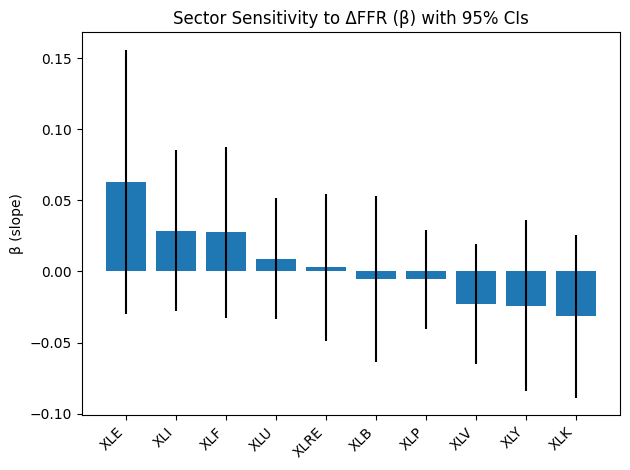
\includegraphics[width=0.8\textwidth]{../figs/sector_sens_to_ffr.png}
    \caption{Sector Sensitivity to Federal Funds Rate Changes With 95\% Confidence Intervals}
    \label{fig:sector_sens}
\end{figure}

\begin{figure}[htbp]
    \centering
    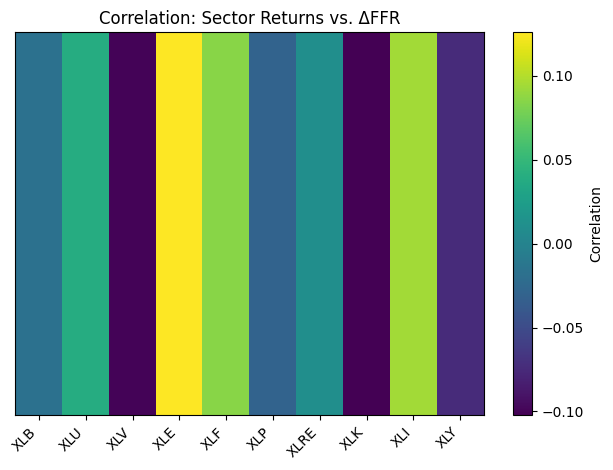
\includegraphics[width=0.8\textwidth]{../figs/sector_return_vs_ffr.png}
    \caption{Sector Returns vs Federal Funds Rate Changes}
    \label{fig:sector_return}
\end{figure}

\begin{figure}[htbp]
    \centering
    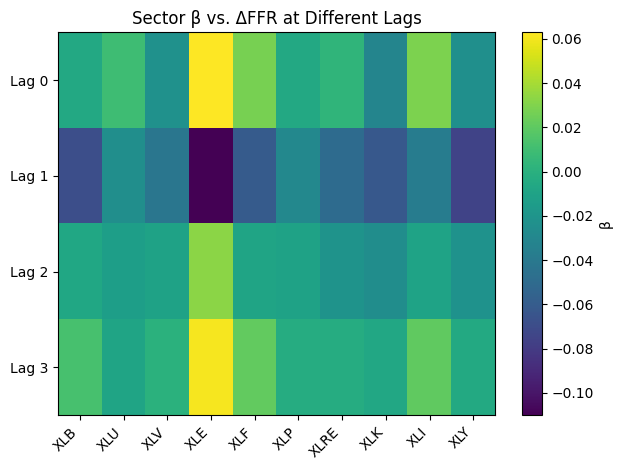
\includegraphics[width=0.8\textwidth]{../figs/sector_beta_vs_ffr_lagged.png}
    \caption{Sector Beta Coefficients with Lagged Federal Funds Rate Changes}
    \label{fig:sector_lagged}
\end{figure}

\begin{figure}[htbp]
    \centering
    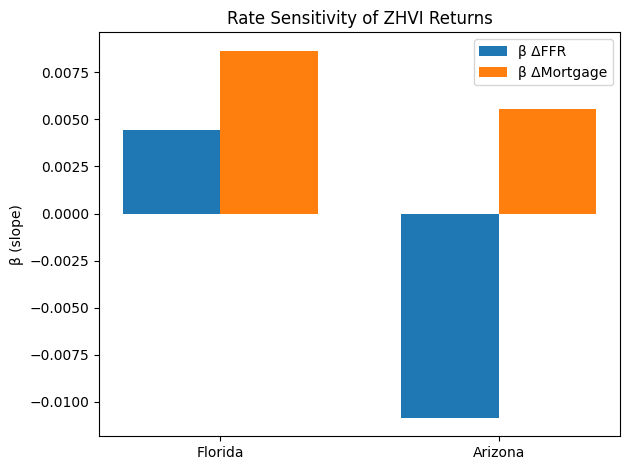
\includegraphics[width=0.8\textwidth]{../figs/rate_sens_zhvi.png}
    \caption{Rate Sensitivity of Zillow Home Value Index}
    \label{fig:zhvi_sens}
\end{figure}

\begin{figure}[htbp]
    \centering
    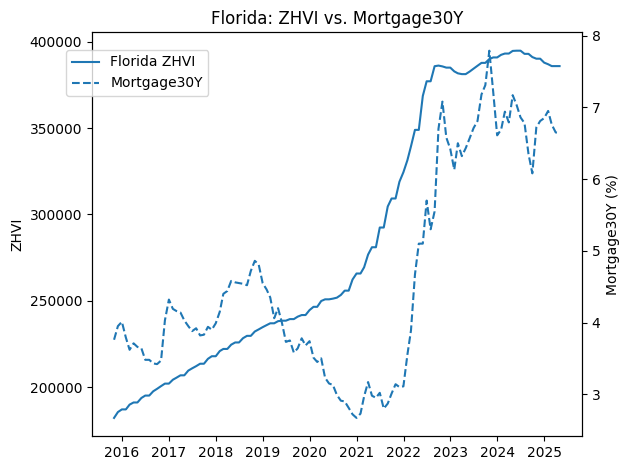
\includegraphics[width=0.8\textwidth]{../figs/fl_zhvi_vs_mort.png}
    \caption{Florida ZHVI vs 30Y Mortgage Rates}
    \label{fig:fl_zhvi}
\end{figure}

\begin{figure}[htbp]
    \centering
    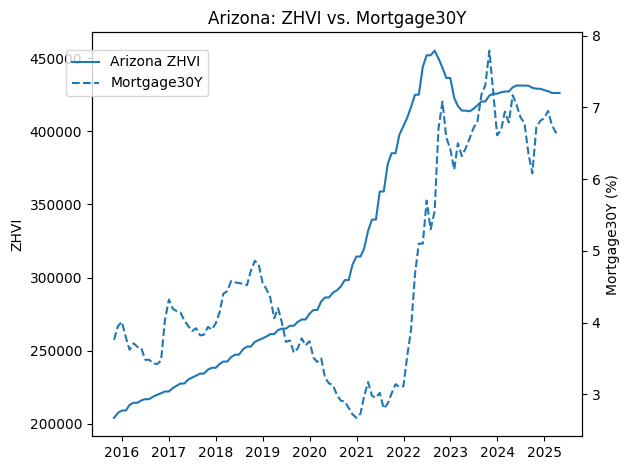
\includegraphics[width=0.8\textwidth]{../figs/az_zhvi_vs_mort.png}
    \caption{Arizona ZHVI vs 30Y Mortgage Rates}
    \label{fig:az_zhvi}
\end{figure}

\begin{figure}[htbp]
    \centering
    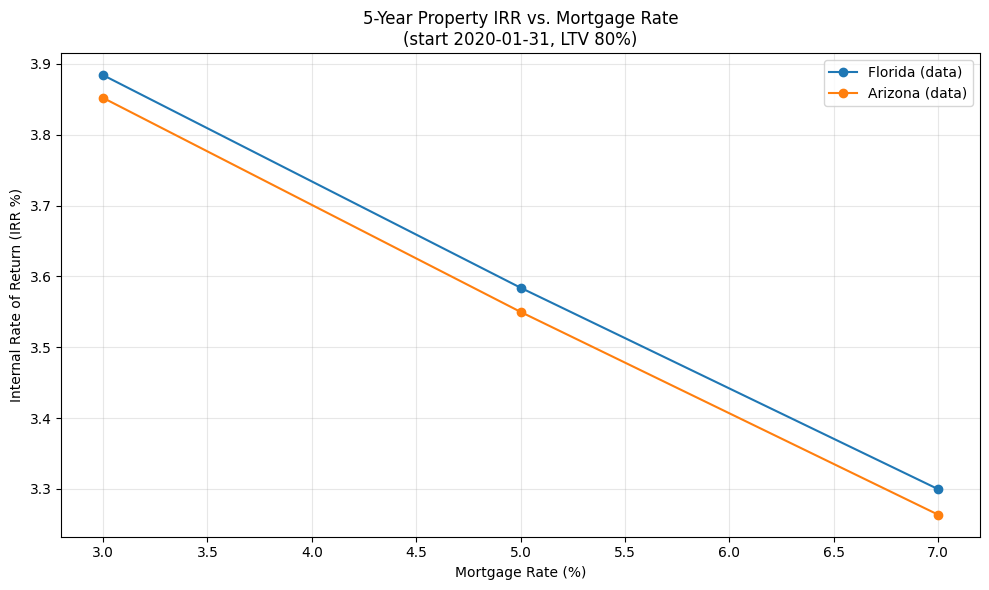
\includegraphics[width=0.8\textwidth]{../figs/irr_vs_mort.png}
    \caption{5-Year IRR vs Mortgage Rates for Florida and Arizona Properties}
    \label{fig:irr_mort}
\end{figure}

\begin{figure}[htbp]
    \centering
    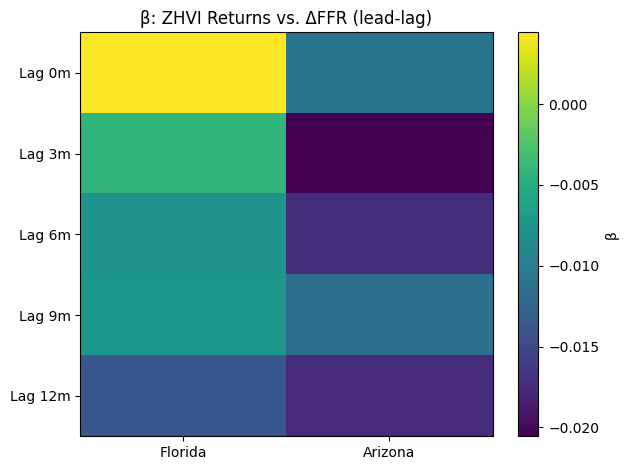
\includegraphics[width=0.8\textwidth]{../figs/zhvi_vs_ffr.png}
    \caption{Zillow Home Value Index vs Federal Funds Rate}
    \label{fig:zhvi_ffr}
\end{figure}

\begin{figure}[htbp]
    \centering
    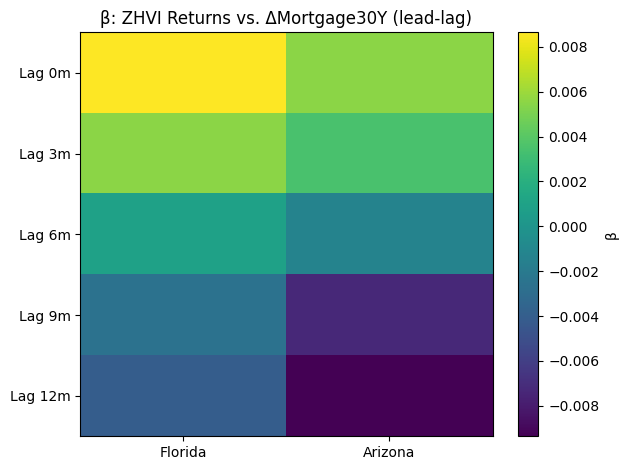
\includegraphics[width=0.8\textwidth]{../figs/zhvi_vs_mort.png}
    \caption{Zillow Home Value Index vs Mortgage Rates}
    \label{fig:zhvi_mort}
\end{figure}

\begin{figure}[htbp]
    \centering
    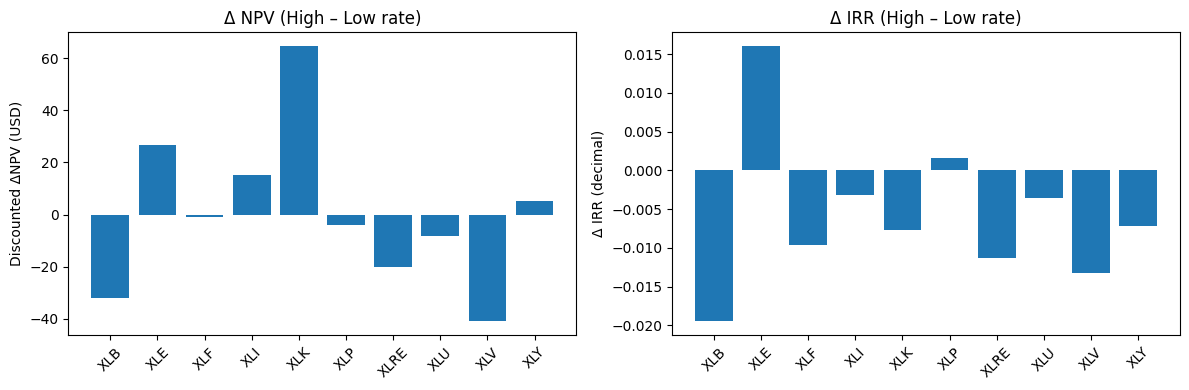
\includegraphics[width=0.8\textwidth]{../figs/npv_iir_sector.png}
    \caption{NPV and IRR Analysis by Sector}
    \label{fig:npv_iir_sector}
\end{figure}

\begin{figure}[htbp]
    \centering
    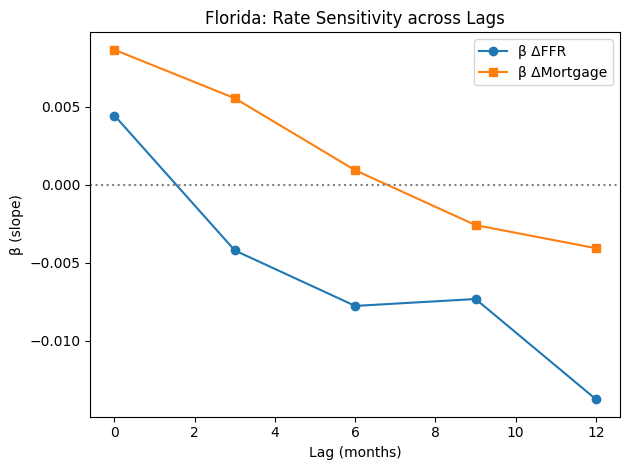
\includegraphics[width=0.8\textwidth]{../figs/fl_rate_sens.png}
    \caption{Florida Rate Sensitivity}
    \label{fig:fl_rate_sens}
\end{figure}

\begin{figure}[htbp]
    \centering
    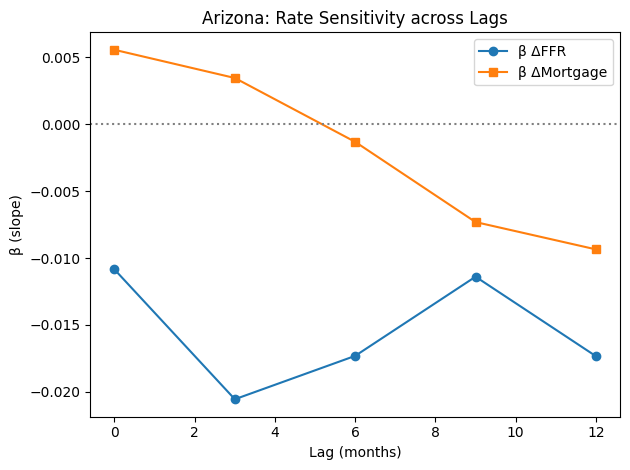
\includegraphics[width=0.8\textwidth]{../figs/az_rate_sens.png}
    \caption{Arizona Rate Sensitivity}
    \label{fig:az_rate_sens}
\end{figure}

\end{appendices}

\end{document}